\documentclass{standalone}
\usepackage[T1]{fontenc}
\usepackage[utf8]{inputenc}
\usepackage{pgf,tikz}
\usepackage{setspace}
\usepackage{pgfplots}
\usepgfplotslibrary{groupplots}
\pgfplotsset{compat=1.13}

\begin{document}

     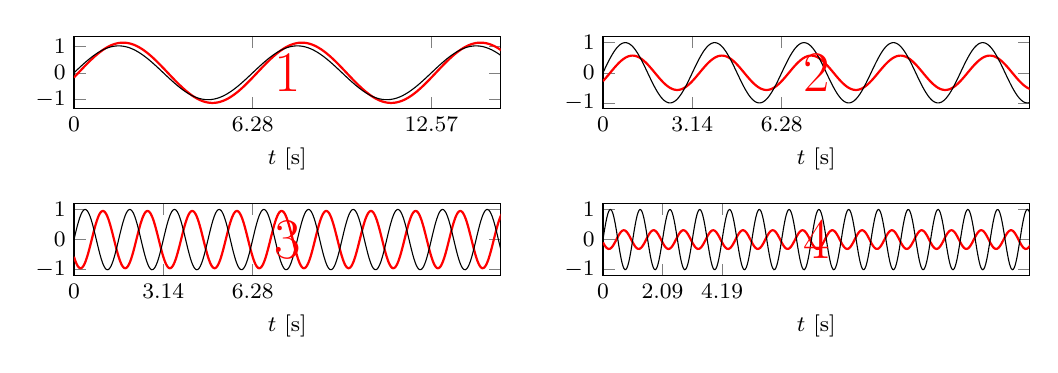
\begin{tikzpicture}
     \footnotesize

     \pgfmathsetmacro{\wwone}{1}
     \pgfmathsetmacro{\wwtwo}{2}
     \pgfmathsetmacro{\wwthree}{4}
     \pgfmathsetmacro{\wwfour}{6}

     \pgfmathsetmacro{\Tone}{2*pi/\wwone}
     \pgfmathsetmacro{\TTone}{2*\Tone}
     \pgfmathsetmacro{\Ttwo}{2*pi/\wwtwo}
     \pgfmathsetmacro{\TTtwo}{2*\Ttwo}
     \pgfmathsetmacro{\Tthree}{4*pi/\wwthree}
     \pgfmathsetmacro{\TTthree}{2*\Tthree}
     \pgfmathsetmacro{\Tfour}{4*pi/\wwfour}
     \pgfmathsetmacro{\TTfour}{2*\Tfour}

     \pgfmathsetmacro{\gainone}{1.12}
     %\pgfmathsetmacro{\gaintwo}{1.67} %true
     \pgfmathsetmacro{\gaintwo}{0.57}
     \pgfmathsetmacro{\gainthree}{0.95}
     \pgfmathsetmacro{\gainfour}{0.31}

     \pgfmathsetmacro{\psone}{-9}
     \pgfmathsetmacro{\pstwo}{-29}
     \pgfmathsetmacro{\psthree}{-143}
     \pgfmathsetmacro{\psfour}{-162}
           
     \begin{groupplot}[group style={group size=2 by 2, vertical sep=1.2cm, horizontal sep=1.3cm},
     width=7cm,
     height=2.5cm,
     xlabel={$t$ [s]},
     %ylabel={$y(t)$},
     xmin=0,
     xmax=15,
     %ytick = \empty,
     %xtick = \empty,
     domain=0:20,
     samples=600,
     variable=t,
     ]

     \nextgroupplot[xtick={0, \Tone, \TTone}]
      \addplot[red, thick, no marks] { \gainone*sin(deg(\wwone*t) + \psone) };
      \addplot[black,  no marks] { sin(deg(\wwone*t)) };

     \nextgroupplot[xtick={0, \Ttwo, \TTtwo}]
      \addplot[red, thick, no marks] { \gaintwo*sin(deg(\wwtwo*t) + \pstwo) };
      \addplot[black,  no marks] { sin(deg(\wwtwo*t)) };
 
     \nextgroupplot[xtick={0, \Tthree, \TTthree}]
      \addplot[red, thick, no marks] { \gainthree*sin(deg(\wwthree*t) + \psthree) };
      \addplot[black,  no marks] { sin(deg(\wwthree*t)) };

     \nextgroupplot[xtick={0, \Tfour, \TTfour}]
      \addplot[red, thick, no marks] { \gainfour*sin(deg(\wwfour*t) + \psfour) };
      \addplot[black,  no marks] { sin(deg(\wwfour*t)) };

     \end{groupplot}

     \node[red] at (group c1r1.center) {\huge 1};
     \node[red] at (group c2r1.center) {\huge 2};
     \node[red] at (group c1r2.center) {\huge 3};
     \node[red] at (group c2r2.center) {\huge 4};
     \end{tikzpicture}

   \end{document}
   